\makeatletter
\long\def\precis#1{%
\@precis{#1}%
\@precistoc{#1}
}

\def\@precis#1{%
\bgroup
\small
\smallskip\parindent0pt
#1\par\medskip\egroup}

\def\@precistoc#1{
\addtocontents{toc}{{\vskip0pt\vbox{\par\color{teal} \smallskip\leftskip15pt\rightskip10pt\parindent0pt\leavevmode #1\par\protect\medskip}}}
}

\chapter{TOC Styling}

\precis{In this chapter we outline a number of experimental keys that been defined to handle Table of Contents (ToC) formatting. These keys are currently experimental.}
\bigskip



\section{Introduction}


\section{Key values}
\keyval{toc levels}{\marg{num}}{sets  the \texttt{tocdepth} counter. If empty no toc is defined. LaTeX uses this to determine how many levels of toc are included.}
\keyval{toc number width}{marg{dimension}}{\cs{@pnumwidth}}
\keyval{toc chapter number color}{}{tocchapternumbercolor@cx}
\keyval{toc chapter number fill}{}{tocchapternumberfill@cx}
\keyval{toc chapter after}{}{tocchapterafter@cx}
\keyval{toc section indent}{}{tocsectionindent@cx}
\keyval{toc subsection indent}{}{tocsubsectionindent@cx}
\keyval{toc subsubsection indent}{}{tocsubsubsectionindent@cx}
\keyval{toc paragraph indent}{}{tocparagraphindent@cx}
\keyval{toc subparagraph indent}{}{tocsubparagraphindent@cx}
\keyval{toc section number width}{}{tocsectionnumberwidth@cx}
\keyval{toc dots}{}{}
\begin{marglist}
 \item[none] this sets the value of \cs{@dotsep} to 1000 thus eliminating the dots.
\item [false] alias for the above key.
\item [true] dot leaders are used, uses a default value for \cs{@dotsep} of 4.5,
\end{marglist}
\keyval{toc dotsep}{\marg{number}}{renewcommand  @dotsep}
\keyval{toc chapter name}{}{chaptername}
\keyval{toc chapter name color}{}{tocchapternamecolor@cx}
\keyval{toc title color}{}{toctitlecolor@cx}
\keyval{toc title font-weight}{}{toctitlefontweight@cx}
\keyval{toc title before}{}{toctitlebefore@cx}
\keyval{toc title after}{}{toctitleafter@cx}
\keyval{toc after pagenumber}{}{tocafterpagenumber@cx}
\keyval{toc right margin}{}{@tocrmarg}
\keyval{toc number after}{}{tocnumberafter@cx}
%  toc number align/.is choice,
%  toc number align/center/.code=\def\tocnumberalign@cx{\centering}\def\stoptocnumberalign@cx{},
%  toc number align/left/.code=\def\tocnumberalign@cx{\centering}\def\stoptocnumberalign@cx{},
%  toc number align/right/.code=\def\tocnumberalign@cx{\hfill}\def\stoptocnumberalign@cx{},
\keyval{toc image}{\marg{filename}}{If the TOC has images associated with chapters these are used in the typesetting. Used with custom templates.}
\keyval{toc custom}{\marg{cmd}}{Triggers the loading of alternative templates than those structured by LaTeX.}
\keyval{hypersetup linkcolor}{\marg{color}}{Changes the color of a hyperlink. This is experimental and better used at document level.}
\keyval{toc chapter precis}{\marg{true|false}}{This is experimental. If a chapter precis is specified in a chapter, then the precis is typeset in the ToC also\footnote{Such a command is provided by the \pkg{tocloft} package and in the memoir class}.}



Firstly we define the width of the box that the page number is set. Use ems so that it does not need to be redefined for every change in font size.
ToC entries are treated as rectangular areas where the text
and probably a filler will be written. Let's draw such an
area (of course, the lines themselves are not printed):



\section{Other Packages and Classes}
The package \pkg{tocloft} provides  provides handles for an author to change the design to meet the needs of the particular document, by providing a number of settings commands.


^^A\addtocontents{toc}{\colorbox{cyan}{\thesection this is some long command \thepage}}

\section{Technical Details}
In the standard classes the design of the Table of Contents (TOC) the List of Figures (lof) and list of tables (lot) is fixed and buried within the class definitions.

To understand the way \LaTeX\ formats the ToC, one has to understand that the ToC entries are generated and typeset in different operations. Firstly when the document is processed, every time a sectioning command such as \cs{chapter} or \cs{section} is activated it calls on either the macro \cs{addcontentsline} or \cs{addcontents}, which in turn will initiate the process of writing the entry onto a file.

The second operation happens when LaTeX sees a \cs{tableofcontents} command. This initiates the read operation, where the information that has been stored in the ToC file is read and typeset.

As the processing for a list of figures and a List of Tables is similar we will only discuss the ToC.


 NOTE: As Peter Wilson says the \pkg{hyperref} package dislikes authors using
\cs{addcontentsline}. To get it to work properly with \pkg{hyperref}  you normally have to put \cs{phantomsection} (a macro defined within  the \pkg{hyperref} package) immediately  before \cs{addcontentsline}. This gave me considerable headaches when redefining these commands for special ToCs.


\section{The \texttt{\textbackslash tableofcontents}}

We should start dissecting the algorithm by first viewing the \cs{tableofcontents}.

\begin{tcolorbox}{}
\begin{lstlisting}
\setcounter{tocdepth}{2}
\newcommand\tableofcontents{%
    \if@twocolumn
      \@restonecoltrue\onecolumn
    \else
      \@restonecolfalse
    \fi
    \chapter*{\contentsname
        \@mkboth{%
           \MakeUppercase\contentsname}{\MakeUppercase\contentsname}}%
          \@starttoc{toc}%
    \if@restonecol\twocolumn\fi
    }
\end{lstlisting}
\end{tcolorbox}

The important thing to notice here is that the words contents are typeset by calling the star version and hence the contents name is not added to the toc. If we needed to add it we need to explicitly add to the toc as well as format it, if necessary. The other notable item is the \cs{starttoc}\marg{toc} macro. This command opens the toc file to read or write.

The macros of a table of contents are saved in an auxiliary file named \marg{jobname.toc} where you can find lines like this:

\subsection{The \texttt{.toc} file}
\subsubsection{The structure of the toc file}

\begin{lstlisting}
\defcounter {refsection}{0}\relax
\contentsline {chapter}{\numberline {1}Table of Contents Styling}{1}{chapter.1}
\defcounter {refsection}{0}\relax
\contentsline {section}{\numberline {1.1}Width of page numbers and a very long and really very long section numbering scheme}{1}{section.1.1}
\defcounter {refsection}{0}\relax
\contentsline {section}{\numberline {1.2}test}{1}{section.1.2}
\defcounter {refsection}{0}\relax
\contentsline {section}{\numberline {1.3}Technical Details}{1}{section.1.3}
\end{lstlisting}
\

When the file is imported back the commands are expanded and the table of contents lines printed as shown below.



\begin{lstlisting}%[title=Extract from .toc file]
\cxset{toc image=false}
\defcounter {refsection}{0}\relax
\contentsline {chapter}{\numberline {1}Table of Contents Styling}{1}{chapter.1}
\defcounter {refsection}{0}\relax
\contentsline {section}{\numberline {1.1}Width of page numbers and a very ong and really very long section numbering scheme}{1}{section.1.1}
\defcounter {refsection}{0}\relax
\contentsline {section}{\numberline {1.2}test}{1}{section.1.2}
\defcounter {refsection}{0}\relax
\contentsline {section}{\numberline {1.3}Technical Details}{1}{section.1.3}
\end{lstlisting}

\subsection{The contentsline and numberline macros}

The two important macros we need to get access to, in order to be able to have a flexible approach in formatting table of contents are \cs{contentsline} and \cs{numberline} and their dependencies.

The \cs{contentsline} definition triggers the calling of macros that start with \verb+l@+ and for the sectioning commands have typical formats such as \lstinline{\l@chapter, \l@section etc.}

\begin{tcolorbox}
\begin{lstlisting}
\def\contentsline#1{\csname l@#1\endcsname}
\end{lstlisting}
\end{tcolorbox}

\subsection{The \textbackslash @starttoc macro}

remember when the tableofcontents was intitiated it called the starttoc command. This is defined in the LaTeX kernel and not in the class files. The \cmd{@starttoc}{hexti} command is used with the commands:
\cs{tableofcontents}, \cs{listoffigures}, etc. \footnote{See a more detailed explanation on ltsect.dtx, page 288.}

For example: \cs{@starttoc}{lof} is used in listoffigures. This command
reads the .ext and sets up to write the new .fil

\begin{tcolorbox}{The @starttoc definition in the LaTeX kernel}
\begin{lstlisting}
\def\@starttoc#1{%
\begingroup
  \makeatletter
  \@input{\jobname.#1}%
  \if@filesw
    \expandafter\newwrite\csname tf@#1\endcsname
    \immediate\openout \csname tf@#1\endcsname \jobname.#1\relax
   \fi
   \@nobreakfalse
\endgroup}
\end{lstlisting}
\end{tcolorbox}

If one had to generate for example mini-toc's this would be difficult if not impossible to achieve. the strategy used by the minitoc package, is to write each chapter toc in an additional subsidiary file, using more or less the same strategy. the information is read in a group so that any formatting information does not affect subsequent sections of the document.

\begin{tcolorbox}
\begin{lstlisting}
\renewcommand*\l@chapter[2]{%
  %#1 number and title  #2 page number
  \ifnum \c@tocdepth >\m@ne
    \addpenalty{-\@highpenalty}%
    \vskip 1.0em \@plus\p@
    \setlength\@tempdima{1.5em}%
    \begingroup
      \parindent \z@ \rightskip \@pnumwidth
      \parfillskip -\@pnumwidth
      \leavevmode \bfseries \color{thegray}
      \advance\leftskip\@tempdima
      \hskip -\leftskip
      (#1)\nobreak\hfil \nobreak\hb@xt@\@pnumwidth{\hss#2\hspace*{3cm}}\par
      \penalty\@highpenalty
    \endgroup
  \fi}

\renewcommand*\l@chapter[2]{%
  %#1 number and title  #2 page number
  \ifnum \c@tocdepth >\m@ne
    \addpenalty{-\@highpenalty}%
    \vskip 1.0em \@plus\p@
    \setlength\@tempdima{1.5em}%
    \begingroup
      \parindent \z@ \rightskip \@pnumwidth
      \parfillskip -\@pnumwidth
      \leavevmode \bfseries \color{thegray}
      \advance\leftskip\@tempdima
      \hskip -\leftskip
      \colorbox{red}{\hbox to 10cm{\color{white}#1\hss #2}}\par
      \penalty\@highpenalty
    \endgroup
  \fi}
\l@chapter{1 test}{12}
\end{lstlisting}
\end{tcolorbox}


So far we have simplistically examined the formatting. Life can get a bit more complex if we want to have a layout as shown in Figure \ref{fig:toc}.

\begin{figure}[tp]
\fbox{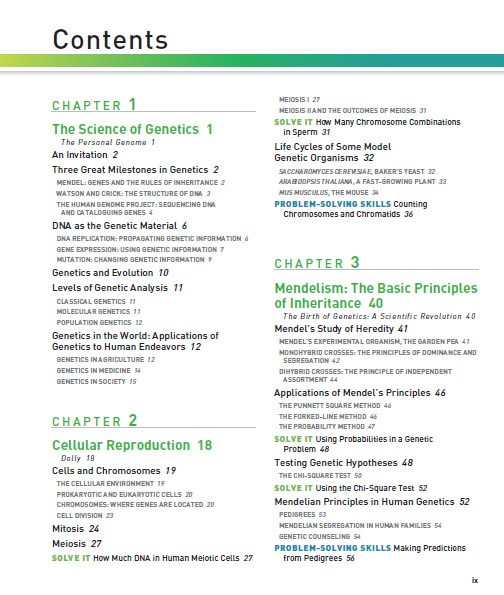
\includegraphics[width=0.5\textwidth]{contents01}}
\caption{Complex table of contents layout.}
\label{fig:toc}
\end{figure}


\begin{lstlisting}
\renewcommand\l@chapter[3]{%
  %#1 number and title  #2 page number
  \ifnum \c@tocdepth >\m@ne
    \addpenalty{-\@highpenalty}%
    \vskip 1.0em \@plus\p@
    \setlength\@tempdima{1.5em}%
    \begingroup
      \parindent \z@ \rightskip \@pnumwidth
      \parfillskip -\@pnumwidth
      \leavevmode
      \advance\leftskip\@tempdima
      \hskip -\leftskip
      \vbox{\raggedright#1\vskip1pt%
      \hrule width3cm height0.4pt}\par
      #2
      \penalty\@highpenalty
    \endgroup
  \fi}
\end{lstlisting}

\begin{lstlisting}
% define three parameters the chapter number, title separate
\renewcommand\l@chapter[3]{%
  %#1 number and title  #2 page number
  \ifnum \c@tocdepth >\m@ne
    \addpenalty{-\@highpenalty}%
    \vskip 1.0em \@plus\p@
    \setlength\@tempdima{1.5em}%
    \begingroup
      \parindent \z@ \rightskip \@pnumwidth
      \parfillskip -\@pnumwidth
      \leavevmode
      \advance\leftskip\@tempdima
      \hskip -\leftskip
      \vbox{\raggedright#1\vskip1pt%
      \hrule width3cm height0.4pt}\par
      #2
      \penalty\@highpenalty
    \endgroup
  \fi}
\cxset{chapter color=thegreen}
\l@chapter{\color{\chaptercolor@cx}\bfseries\chaptername\hskip1em\thechapter}{A Chapter Title}{12}
\end{lstlisting}


In this figure only the chapter number is shown, no page number and the section details are layed down in a two column format.


If we take a similarly flexible approach of redefining l@chapter we can try and format the toc shown in Figure \ref{fig:tocsteward}.

\begin{figure}[tp]
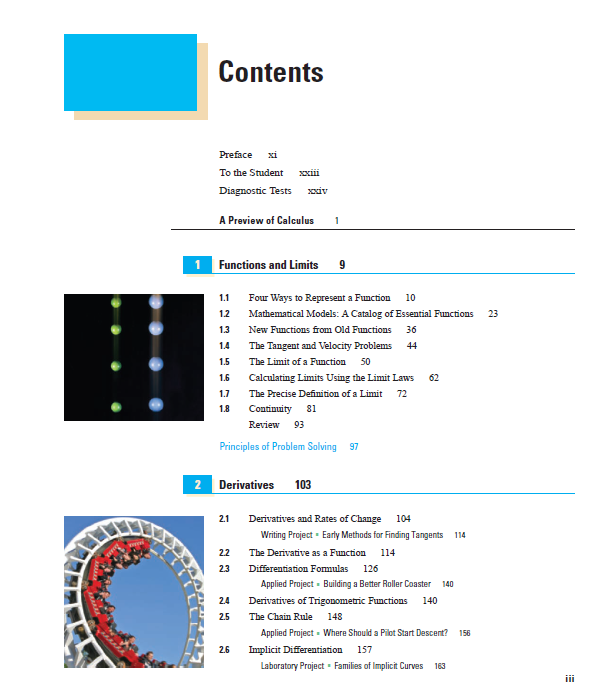
\includegraphics[width=0.8\textwidth]{contents02}
\caption{Complex table of contents layout.}
\label{fig:tocsteward}
\end{figure}



\begin{lstlisting}
\renewcommand\l@chapter[3]{%
  %#1 number and title  #2 page number
  \ifnum \c@tocdepth >\m@ne
    \addpenalty{-\@highpenalty}%
    \vskip 1.0em \@plus\p@
    \begingroup
      \parindent \z@
      \leavevmode
      \vbox{\raggedright\colorbox{blue}{\color{white}\bfseries\sffamily#1} #2\qquad  #3\vskip0pt%
      \color{blue}\hrule width0.7\textwidth height0.4pt}\par
      \penalty\@highpenalty
    \endgroup
  \fi}
\end{lstlisting}

\begin{lstlisting}
% define three parameters the chapter number, title separate
\cxset{
  toc chapter name/.store in=\chaptername,
  toc chapter name color/.code=\gdef\tocchapternamecolor@cx{#1},
  toc title color/.store in=\toctitlecolor@cx,
  toc title font-weight/.store in=\toctitlefontweight@cx,
  toc title before/.store in=\toctitlebefore@cx,
  toc title after/.store in=\toctitleafter@cx,
  toc after pagenumber/.store in=\tocafterpagenumber@cx,
}
\cxset{toc title color=theblue,  %interfers with links
       toc title font-weight=\fontfamily{ptm}\selectfont\bfseries ,
       toc title before=\hspace*{0.5em},
       toc title after=\hspace*{1.5em},
       toc after pagenumber=,
}
\renewcommand\l@chapter[3]{%
% #1 number #2
%  title  #2 page number
  \ifnum \c@tocdepth >\m@ne
    \addpenalty{-\@highpenalty}%
    \vskip 1.0em \@plus\p@
    \begingroup
      \parindent \z@
      \leavevmode
      \vbox{\raggedright\colorbox{blue}{\color{white}%
             \sffamily#1 }%
%% title formatting
        {\toctitlebefore@cx\color\toctitlecolor@cx\toctitlefontweight@cx%
          #2%
          \toctitleafter@cx}% font info
          #3\tocafterpagenumber@cx\vskip0pt%
              \color{blue}
              \hrule width0.7\textwidth height0.4pt}\par
      \penalty\@highpenalty
    \endgroup
  \fi}

\cxset{chapter color=thegreen}
\l@chapter{12}{A Chapter Title}{\thepage}%where is page number coming?numberline

\l@chapter{12}{A Chapter Title}{\thepage}
\end{lstlisting}


The above method of redefinition is a bit more flexible and can be extended to cover all cases that do not fall broadly with the standard class provisions.


\section{Writing the Table of Contents Entries}


One needs to keep in mind that there are two distinct operations in typesetting a ToC. The first one is the writing of the necessary information to the aux file. The second one is the operations that happen when the file is read in a series of instructions triggered by the \cs{tableofcontents} command.

If we have to ensure that information survives we need to wrie it to the file. This is done via two macros.
The \cs{addcontentsline}\marg{table}\marg{type}\marg{entry} command allows the user to add an entry to a table of contents. The command adds the entry
\cs{contentsline}\marg{type}\marg{entry}\marg{page} to the \marg{.table} file.

\begin{lstlisting}
 \addcontentsline{toc}{chapter}%
       {\protect\numberline{\thechapter}#1}

\def\addcontentsline#1#2#3{%
  \addtocontents{#1}{\protect\contentsline{#2}{#3}{\thepage}}}

\def\contentsline#1{\csname l@#1\endcsname}
\end{lstlisting}

The entries for this document with fancy chapter formatting end in the .toc file as:
\begin{lstlisting}
 \addcontentsline{toc}{chapter} {%
      \protect\numberline{%
           \colorbox{\protect\tocchapternumberfill@cx}{\color{\tocchapternumbercolor@cx}%
                \string\parbox{1.5em}%
                {\protect\tocnumberalign@cx\thechapter
                 \stoptocnumberalign@cx}}%
                \Rule\kern-13cm\hspace{1em}\bfseries\sffamily\MakeUppercase{#2}
     }
}
\end{lstlisting}


\section{Approach to defining appropriate hooks}

In order to introduce the appropriate hooks for the various formatting commands two approaches were considered. One was to add images and special formatting via additional addcontents lines in the chapter definitions. This works well for items such as triggering the addition of a chapter precis, or images before chapter headings. The second approach was to add hooks withing the arguments to numberline and contentsline. This works well with fonts formatting and spacing commands but is difficult to achieve due to the information lying in more than one place. Another experimental approach is to save the values of the information only, so once you are reading the file you can feed it into a typesetter type of command. In my opinion this is the best way, it can work well with chapters and parts, but for sections it presents difficulties as we are touhing the kernel. I tried very hard not to modify any kernel commands. Class commands are ok to redefine within reason but the kernel should be left untouched.

The approach save values for the following in a file.

\begin{lstlisting}
while not eof do
    tocline{chapternumber,chaptertitle,pagenumber,others,....,
               values for formatting.}
    format and print the line as per the information read.
endwhile
\end{lstlisting}

Typesetting rules require consistency and therefore it is not all that hard.

If special toc design DO NOT CALL l@section but call l@section@special

\begin{lstlisting}
\def\contentsline#1{\csname l@#1\endcsname}
\def\numberline#1{\hb@xt@\@tempdima{#1\hfil}}
\l@chapter{}{}{}
%% The contents line results in
\l@chapter{\numberline {1}First}{1}
\end{lstlisting}
